\documentclass[11pt,a4paper]{article}
\usepackage[margin=2.4cm]{geometry}
\usepackage[T1]{fontenc}
\usepackage{lmodern}
\usepackage{microtype}
\usepackage{booktabs}
\usepackage{tabularx}
\usepackage{array}
\usepackage{xcolor}
\usepackage{tikz}
\usetikzlibrary{arrows.meta,positioning,calc}
\usepackage{enumitem}
\usepackage{titlesec}
\usepackage{fancyhdr}
\usepackage[hidelinks]{hyperref}

\definecolor{teal}{HTML}{0F6B78}
\titleformat{\section}{\Large\bfseries\color{teal}}{\thesection}{0.6em}{}
\titleformat{\subsection}{\large\bfseries}{\thesubsection}{0.6em}{}
\setlist{nosep,leftmargin=1.4em}
\setlength{\parindent}{0pt}
\setlength{\parskip}{0.55em}
\renewcommand{\arraystretch}{1.18}
\pagestyle{fancy}
\fancyhf{}
\renewcommand{\headrulewidth}{0pt}
\fancyfoot[L]{\footnotesize NABD technical documentation (draft for review)}
\fancyfoot[R]{\footnotesize\thepage}
\newcolumntype{Y}{>{\raggedright\arraybackslash}X}

\begin{document}

\begin{flushleft}
{\Huge\bfseries NABD}\\[0.3em]
{\Large Technical documentation: probabilistic RSV and influenza forecasts for the UAE}\\[0.8em]
{\small Future Health Digital Innovation Challenge 2026 \textperiodcentered{} Statement 06, Population and Workforce Health Early Warning\\
Ammad Hassan (sole entrant), MBZUAI \textperiodcentered{} Draft for early review, 15 November 2026\\
Repository: \url{https://github.com/Ammad1H/NABD}}
\end{flushleft}

\begin{abstract}
\noindent NABD forecasts the weekly share of laboratory samples that test positive for RSV and for influenza in the United Arab Emirates, three weeks ahead, as probabilistic ranges rather than single numbers. Each forecast is turned into the chance of crossing a pressure threshold and into one proposed action for a named role, which a person approves, modifies or dismisses. The UAE's public surveillance record is only four seasons long, which is too short for a model built on it alone to beat the simple rule of repeating last week. NABD therefore trains one model on the WHO surveillance histories of many countries and applies it to a country that brings only its recent weeks. On eighteen countries that were held out under a pre-registered plan, this pooled model made 23\% less influenza forecast error than a model fitted to each country's own record. The work is a prototype on public data. No hospital has used it, and this document states what has and has not been shown.
\end{abstract}

\section{Problem and scope}

Every winter, RSV and influenza reach children's wards in Abu Dhabi at the same time. Bed managers, public-health duty officers and the immunisation programme plan the next few weeks largely from last week's numbers and last year's pattern. UAE seasons change in timing and shape from year to year: influenza peaked at 40.6\% positivity in October 2025, after a five-month plateau that peaked in February the season before, and the RSV peak has moved between ISO weeks 41 and 47. One Abu Dhabi hospital recorded 2,189 RSV admissions of children aged five or under between 2018 and 2022.

NABD is meant to sit on top of existing detection systems as a forecast layer. It forecasts how high and how long a season will run. It does not claim to detect the start of a surge earlier than a hospital's own census would. It forecasts laboratory positivity, which is not hospital load; whether the two move together closely enough to matter operationally is an open assumption (Section~\ref{sec:assumptions}) and the question a pilot would answer.

\section{Data}

The forecasts use weekly aggregates only. The primary source is WHO FluNet, accessed through the WHO xMart interface: sentinel positivity and testing volume for the UAE, and the equivalent series for 46 development countries and 18 held-out countries. Oman, Qatar and Saudi Arabia form a separate Gulf test. The United States benchmark uses the CDC FluSight hub, including its archived forecasts from other models. School calendars and Ramadan dates are used by one challenger model. Every adapter validates its input against a schema that rejects person-level fields, and the pilot specification adds suppression of any cell below ten.

Two properties of the data matter for interpretation. WHO publishes each week with a lag of roughly seven to eleven days, so the horizons are defined from the issue date. And retrospective tests necessarily use revised values, because no real-time vintages of FluNet exist; this flatters the retrospective results relative to live use, which is the reason a live test was added.

\section{System architecture}

Figure~\ref{fig:arch} shows the pipeline. Models write forecasts in the CDC FluSight quantile format (23 quantile levels), so any model, front-end or scorer can read any forecast file. Each weekly round of forecasts is hashed before WHO publishes the week it covers. The web page, the Streamlit workbench and the API all read results through a single loader, so they cannot disagree on a number.

\begin{figure}[h]
\centering
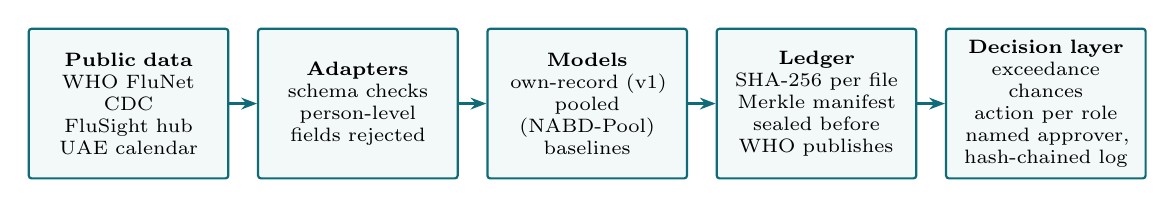
\begin{tikzpicture}[
  box/.style={draw=teal, thick, rounded corners=1pt, minimum width=2.45cm, minimum height=1.9cm, align=center, font=\scriptsize, text width=2.3cm, fill=teal!5},
  arr/.style={-{Stealth[length=2mm]}, thick, teal}]
  \node[box] (a) {\textbf{Public data}\\WHO FluNet\\CDC FluSight hub\\UAE calendar};
  \node[box, right=0.35cm of a] (b) {\textbf{Adapters}\\schema checks\\person-level fields rejected};
  \node[box, right=0.35cm of b] (c) {\textbf{Models}\\own-record (v1)\\pooled (NABD-Pool)\\baselines};
  \node[box, right=0.35cm of c] (d) {\textbf{Ledger}\\SHA-256 per file\\Merkle manifest\\sealed before WHO publishes};
  \node[box, right=0.35cm of d] (e) {\textbf{Decision layer}\\exceedance chances\\action per role\\named approver, hash-chained log};
  \draw[arr] (a)--(b); \draw[arr] (b)--(c); \draw[arr] (c)--(d); \draw[arr] (d)--(e);
\end{tikzpicture}
\caption{NABD pipeline. Locked evaluations (held-out countries, Gulf, United States, live UAE test) read the same forecast files. Interfaces: a static bilingual web page, a Streamlit workbench, a FastAPI \texttt{/forecast} endpoint and a weekly PDF bulletin.}
\label{fig:arch}
\end{figure}

\section{Models}

\subsection{Own-record model (NABD-UAE-v1)}
The headline model is a pooled linear growth model on the logit scale with a seasonal-climatology term, using only the UAE sentinel positivity and testing volume. Its prediction intervals come from nested out-of-season residuals. The model was frozen at a recorded commit before the evaluations reported here, and it remains the headline model of the live ledger.

\subsection{Pooled model (NABD-Pool)}
The pooled model is built around borrowed strength: a country with a short record is forecast from many countries' histories rather than its own alone. It predicts the within-season change in logit positivity at horizons of one to four weeks and outputs the 23 FluSight quantiles. It is the quantile average of two members. The first is a gradient-boosted quantile model, one fit per quantile level, trained across all countries and horizons, with features describing the country's own recent lags and growth, its deviation from its own past-season pattern, season phase, latitude and hemisphere, testing volume and the number of earlier seasons available. The second is the own-record model's linear form with coefficients fitted on pooled rows and shrunk towards the country's own fit with weight $n/(n+8)$, where $n$ is the number of the country's own earlier seasons. Model selection used the 46 development countries only, forward in time and with the target country left out of each fit. For a held-out country the model sees that country's data up to the forecast origin and nothing later, which is the same information the own-record method has. It runs on a laptop CPU in seconds, and every forecast decomposes exactly into its inputs.

\subsection{Comparators}
The reference forecasts are repeating last week's value and the pattern of past seasons. A multi-signal variant of the own-record model (NABD-UAE-v2) adds non-sentinel positivity, school breaks and Ramadan. A United States ensemble, an equal-weight quantile average of a damped log-linear negative-binomial model and an empirical error model, is used only to stress-test the method against the CDC FluSight ensemble. A general time-series foundation model (\texttt{amazon/\allowbreak chronos-2}) was run zero-shot on the held-out forecasts as an outside benchmark; it is never an input to NABD.

\section{Evaluation protocol and integrity}

Forecasts are scored with the weighted interval score (WIS) \cite{bracher2021}, a proper scoring rule \cite{gneiting2007}. Results are reported as the ratio of one model's mean WIS to another's, so a value below one means the first model made less error. Confidence intervals come from a bootstrap that resamples countries, not individual forecasts, because forecasts within a country are strongly dependent.

The evaluations that carry weight were fixed before their data were opened. For the held-out test, the plan was committed with a hash manifest before any held-out data were downloaded, and the pooled model was committed before a single held-out row was extracted; the test was then scored once. The code refuses to score if a locked file has changed. Any analysis added afterwards is recorded in \texttt{docs/DEVIATIONS.md} before it is run and labelled post hoc. A limit on this scheme should be stated plainly: the locks are commits in a git repository, which is self-attested until the fingerprints are stamped by an independent timestamp service. That anchoring step has not been done yet.

For live use, each weekly round of forecasts is written to files, each with a SHA-256 digest and a Merkle manifest, before WHO publishes the target week, and is scored once the week appears. The web page recomputes the digests in the browser. A prospective UAE test comparing the pooled model with the own-record model across the 2026/27 season was locked before its first data point; it is assessed once, on or after 15 April 2027. As of this draft, three rounds have been issued and no target week has yet been published, so no live week has been scored.

\section{Results}

Table~\ref{tab:results} lists every test that has been run, including the ones that did not go in the model's favour, together with its status.

\begin{table}[h]
\centering
\small
\begin{tabularx}{\textwidth}{@{}>{\raggedright\arraybackslash}p{3.6cm}Y>{\raggedright\arraybackslash}p{2.7cm}@{}}
\toprule
Test & Result & Status \\
\midrule
Eighteen held-out countries, influenza & Pooled model against each country's own-record model: 0.767 (95\% CI 0.681--0.832), better in all 18; 0.624 where the country had two or fewer earlier seasons; against repeating last week, 0.879 & Pre-registered; primary criterion met \\
Gulf: Oman, Qatar, Saudi Arabia & Own-record model against last week: 0.914 (0.843--0.983); against past-season pattern: 0.536 & Pre-registered; primary criterion met \\
United States against the CDC FluSight ensemble & 1.22 (1.01--1.52) against a pre-set bar of 1.15; seventh of 21 and nineteenth of 25 single models in the two seasons & Pre-registered; \textbf{not met} \\
UAE's own record, forward in time & Own-record model against last week: 1.002, a tie, on four seasons & Retrospective \\
Foundation model, same forecasts & Chronos-2 zero-shot against the pooled model: 1.026 (0.993--1.055); against own-record model: 0.787 & Post hoc \\
Roster-rule replay & Mis-rostered weeks per season: pooled 10.5, own-record 12.3, last week 11.1, past pattern 16.6; pooled against last week not distinguishable & Post hoc \\
Live UAE test & Pooled against own-record model, season 2026/27; no result before April 2027 & Pre-registered; pending \\
\bottomrule
\end{tabularx}
\caption{Results by test. Ratios are relative WIS; below 1 favours the first-named model.}
\label{tab:results}
\end{table}

Two readings deserve emphasis. The pooled model's advantage over the own-record model is large, consistent across countries and largest where the record is short, which is the UAE's position. But the evidence comes from other countries; UAE data had been examined before these tests, so a confirmatory UAE result can only come forward in time. And the gain does not carry cleanly into decisions: in the roster replay the pooled model is better than the own-record model and much better than planning from past seasons, but it is not distinguishable from repeating last week at that horizon.

\section{Decision layer and governance}

The weekly card shows the forecast as a fan of ranges, always beside the repeat-last-week forecast as a guard against over-trusting the model. From the issued quantiles it computes the probability that each future week exceeds each threshold, and it selects a playbook band from the highest threshold whose probability reaches 30\% together with the direction of the forecast. A consistency check blocks any card whose band, trend and action contradict one another. The playbook thresholds and wording are illustrative placeholders until a clinician and a public-health officer review them.

Nothing is communicated automatically. A named approver chooses to approve, modify or dismiss each proposed action and must give a reason code. Each decision is appended to a log in which every record carries the hash of the previous one, so an edit anywhere in the history is detectable. The system handles aggregate data only. A hospital-planning view translates a forecast into beds and staff from figures the hospital supplies, and it is labelled as a scenario. An employer-absence feed is a simulated design on synthetic data and is marked as such wherever it appears.

\section{Assumptions, dependencies and limitations}
\label{sec:assumptions}

\textbf{Assumptions.} WHO sentinel positivity is taken to indicate community activity, although testing practice can change. Publication lag is assumed to be about seven to eleven days. Retrospective results rest on revised data. Most importantly, hospital load is assumed to follow community positivity closely enough for a positivity forecast to be useful in operations; this has not been tested and is the central question for a pilot. The playbook is assumed to be adjustable by clinical reviewers.

\textbf{Dependencies.} The data come from WHO FluNet, used under its public-health, non-commercial terms, from the CDC FluSight hub, and from public UAE school calendars. The software is Python 3.12 with pandas, scikit-learn, statsmodels, Streamlit and FastAPI, and runs on a CPU. The foundation-model benchmark is optional and needs a deep-learning library and access to the model weights. A pilot needs one hospital's aggregate weekly paediatric respiratory counts under a data-sharing agreement.

\textbf{Limitations.}
\begin{itemize}
\item In the United States, NABD missed its own pre-registered bar against the CDC's combined forecast.
\item A model trained on the UAE's four-season record alone only ties repeating last week; adding non-sentinel and calendar signals did not improve it.
\item The method forecasts size and duration. It does not give earlier warning of onset.
\item No Abu Dhabi hospital, district or daily data have been used, so no operational claim is made.
\item Lock and ledger times are self-attested until the repository is anchored with an external timestamp service, and the hosted demonstration link is not yet live.
\item Forecasts are of laboratory positivity and inherit the reporting delays and revisions of the source.
\end{itemize}

\section{Reproducing the work}

The repository contains the code, the locked plans with their manifests, every result table and 157 automated tests covering adapters, leakage and future-perturbation checks, the locks, the card consistency check, the audit chain, the ledger and the web build. After \texttt{pip install -r requirements-dev.txt}, the command \texttt{pytest -q} runs the suite, \texttt{python -m web.build} regenerates the web page from the result files, \texttt{streamlit run app/streamlit\_app.py} starts the workbench, and \texttt{python -m ledger.weekly --fetch --with-pool} pulls new WHO data, scores past rounds and issues a new round when data are available. The longer technical description is \texttt{docs/TECHNICAL.md}, claims are governed by \texttt{research/claims-ledger.md}, and every deviation from a locked plan is in \texttt{docs/DEVIATIONS.md}.

\section{Where architectural feedback would help}

Four questions would most improve the next iteration. First, whether a positivity forecast is the right interface for hospital operations, or whether a pilot should target admissions directly once a hospital's counts exist. Second, how a pooled model should be governed in production, including retraining cadence, drift monitoring and the conditions under which a challenger may replace the headline model. Third, what the integration path would look like for a read-only forecast feed with a human approval step inside existing Abu Dhabi systems. Fourth, whether a locked live test followed by a twelve-week shadow pilot with a pre-set exit criterion is the right shape for a first deployment.

\begin{thebibliography}{9}
\bibitem{bracher2021} J.~Bracher, E.~L.~Ray, T.~Gneiting and N.~G.~Reich. Evaluating epidemic forecasts in an interval format. \emph{PLOS Computational Biology}, 17(2):e1008618, 2021.
\bibitem{gneiting2007} T.~Gneiting and A.~E.~Raftery. Strictly proper scoring rules, prediction, and estimation. \emph{Journal of the American Statistical Association}, 102(477):359--378, 2007.
\bibitem{flunet} World Health Organization. FluNet: global influenza surveillance and response system. Weekly surveillance data, accessed November 2026.
\bibitem{flusight} Centers for Disease Control and Prevention. FluSight forecast hub. Archived forecasts and NHSN admissions data, accessed November 2026.
\end{thebibliography}

\end{document}
